\chapter{Resultados processamento de imagem }

Características do computador 
\begin{itemize}
	\item CPU: Intel Core i7-3630QM CPU @ 2.40GHz x 8
	\item SO version: Ubuntu 16.04.2 LTS
	\item Intel Corporation 3rd Gen Core processor Graphics Controller (rev 09)
	NVIDIA Corporation GF108M [GeForce GT 635M] (rev a1)
\end{itemize}

%Intel® Core™ i7-3630QM CPU @ 2.40GHz × 8


\newpage
\section{Frame 1}


Características: 
\begin{itemize}
	\item \textbf{Extensão}: .png
	\item \textbf{Tamanho (MB)}: 1.3
	\item \textbf{Dimensões (px)}: 1366 x 768
	\item \textbf{Número de pessoas existentes: } : 17
\end{itemize}


\begin{figure}[!htb]
	\centering
	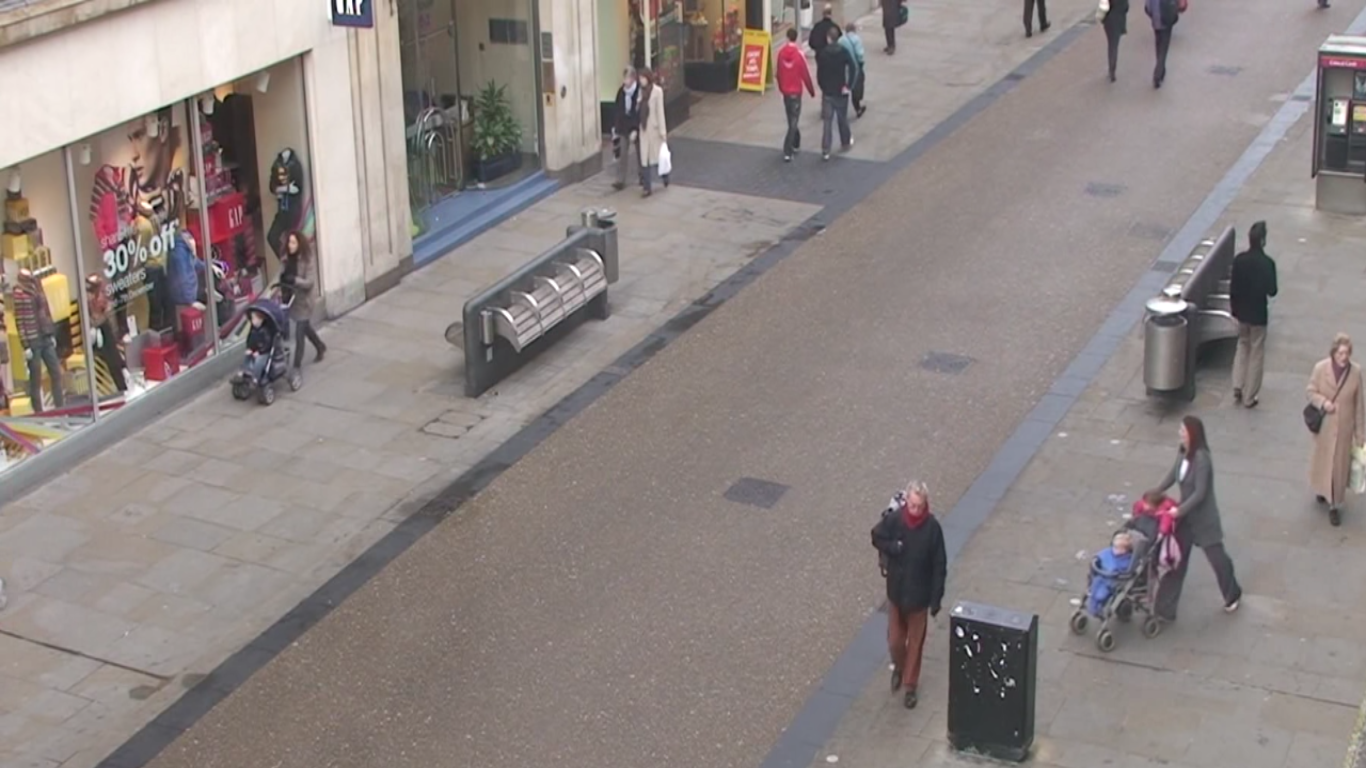
\includegraphics[width=\linewidth]{img/vision/frame1.png}
	\caption{Pirâmide do conhecimento: modelo DIKW}
	\label{db}
\end{figure}



\newpage
\section{Frame 2}

Características: 
\begin{itemize}
	\item \textbf{Extensão}: .png
	\item \textbf{Tamanho (MB)}: 1.2
	\item \textbf{Dimensões (px)}: 1366 x 768
	\item \textbf{Número de pessoas existentes: } : 18
\end{itemize}


\begin{figure}[!htb]
	\centering
	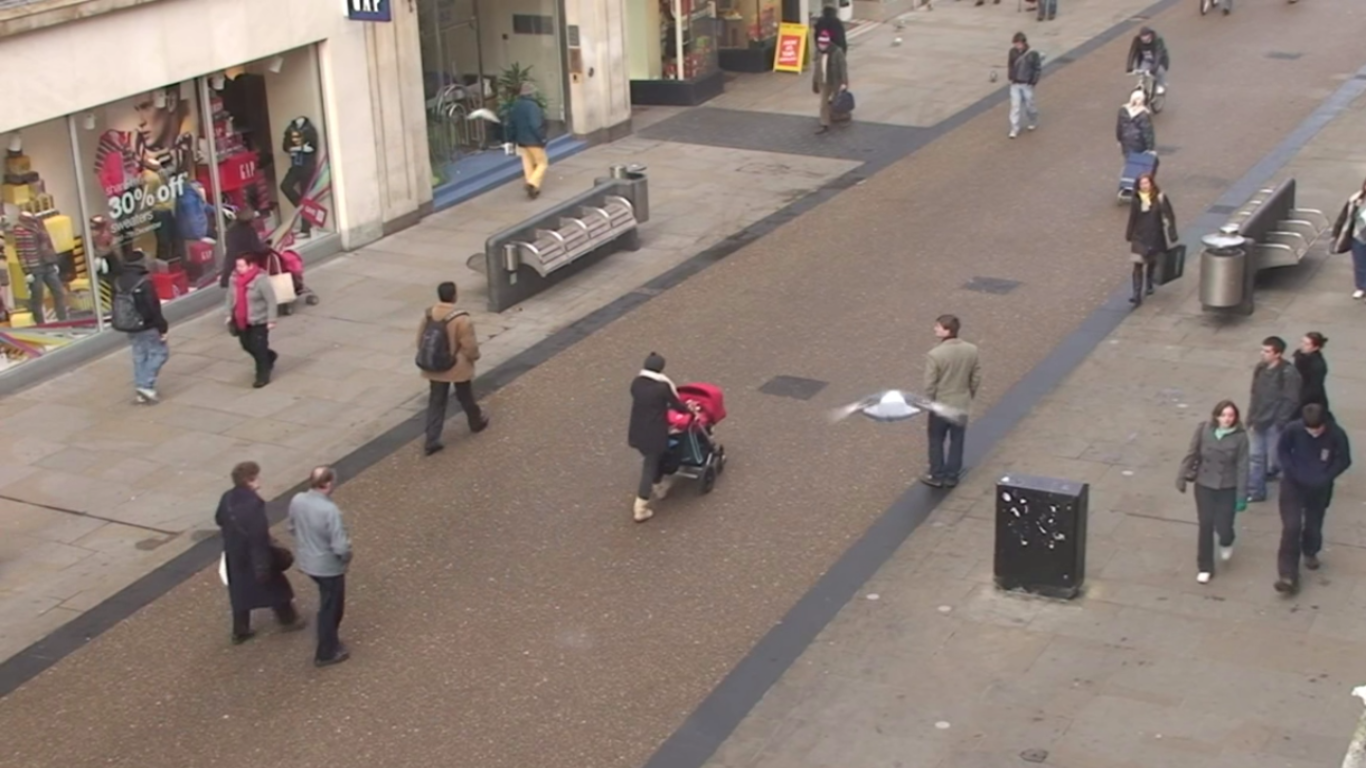
\includegraphics[width=\linewidth]{img/vision/frame2.png}
	\caption{Pirâmide do conhecimento: modelo DIKW}
	\label{db}
\end{figure}



\begin{longtable}{|l|l|l|l|l|l|} 
\hline
\textbf{winStride} & \textbf{padding} & \textbf{scale} & \textbf{detection (number)} & \textbf{execution time (seg)} \\ \hline
(e
(2, 2) & (24, 24) & 0.9 & 7 & 1.38025999069 \\ \hline

	\caption{Your caption here} % needs to go inside longtable environment
	\label{tab:myfirstlongtable}
\end{longtable}





\newpage
\section{Frame 3}


\begin{figure}[!htb]
	\centering
	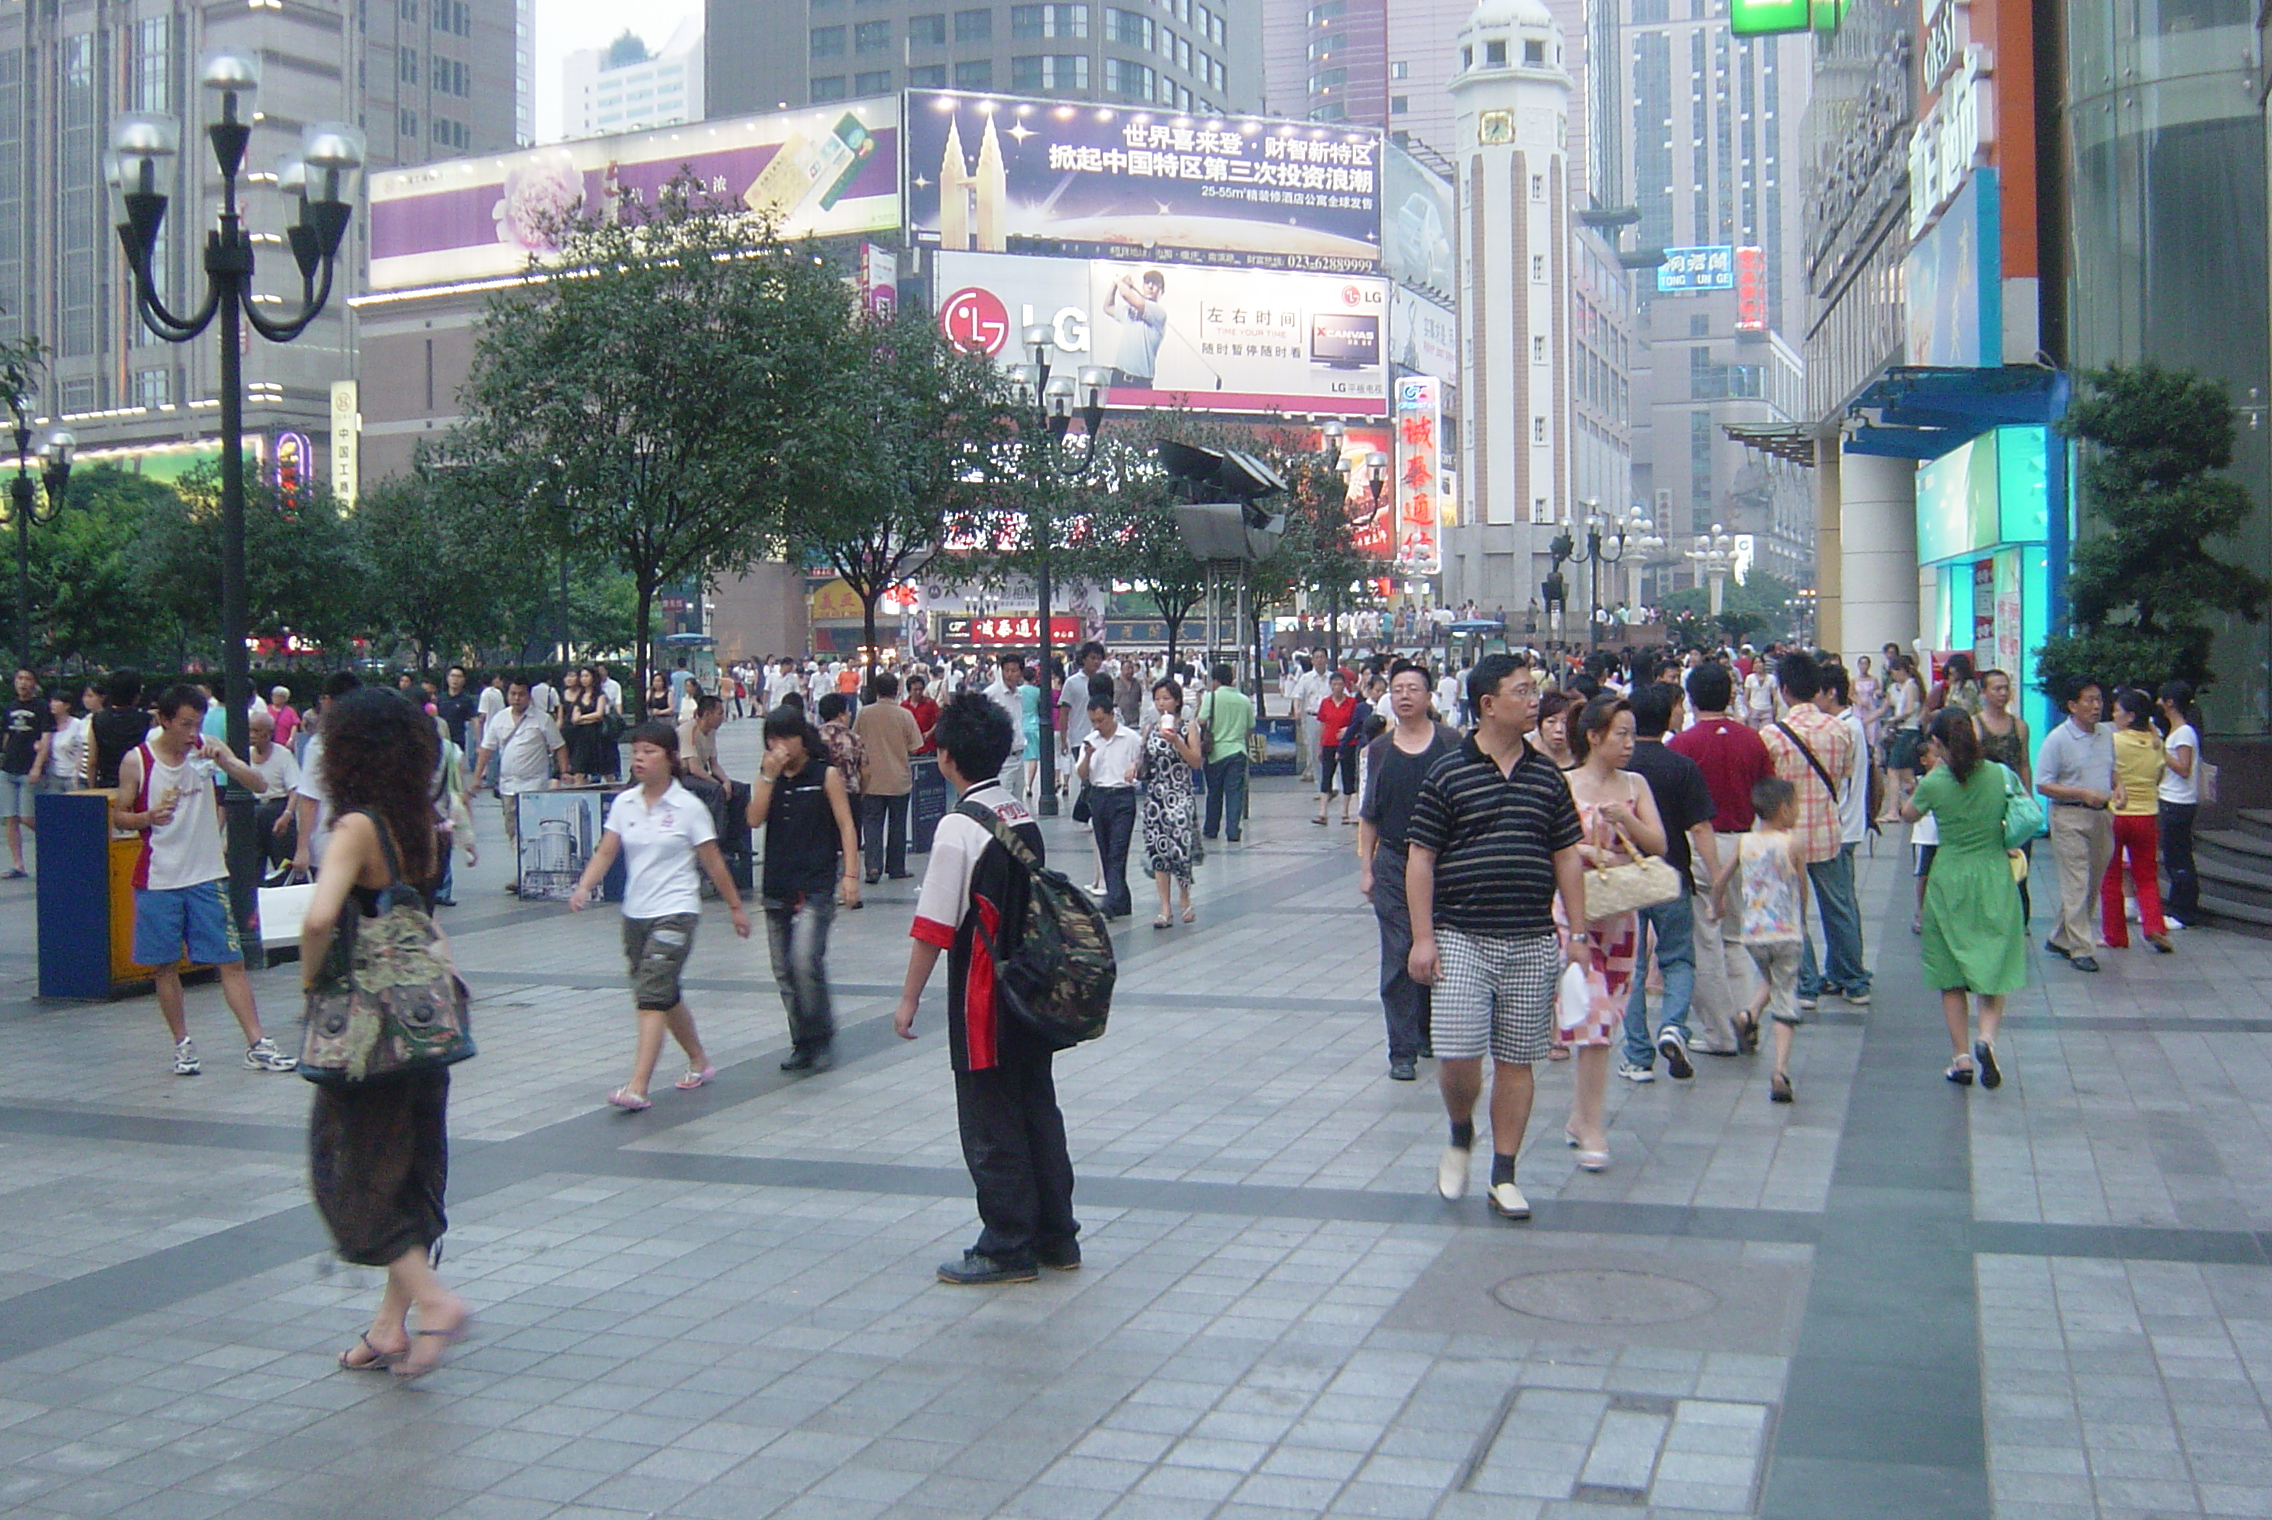
\includegraphics[width=\linewidth]{img/vision/frame3.JPG}
	\caption{Pirâmide do conhecimento: modelo DIKW}
	\label{db}
\end{figure}

Características: 
\begin{itemize}
	\item \textbf{Extensão}: .png
	\item \textbf{Tamanho (MB)}: 1.2
	\item \textbf{Dimensões (px)}: 1366 x 768
\end{itemize}

\begin{table}[h]
	\centering
	\begin{tabular}{|l|l|l|l|l|l|}
		\hline
		\textbf{file} & \textbf{winStride} & \textbf{padding} & \textbf{scale} & \textbf{detection (number)} & \textbf{time (seg)} \\ \hline
		take2.avi & (2, 2) & (8, 8) & 0.5 & 7909 & 404.363101959 \\ \hline
		
		
	\end{tabular}
	\caption{My caption}
	\label{my-label}
\end{table}






\newpage
\section{Frame 4}




\begin{figure}[!htb]
	\centering
	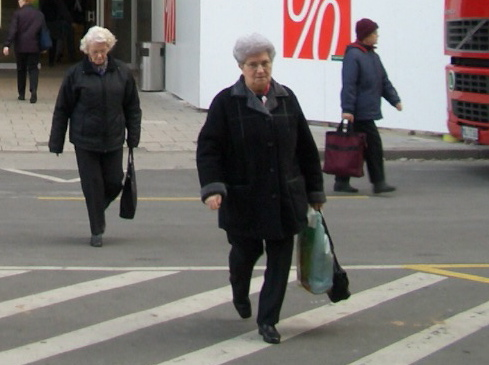
\includegraphics[width=\linewidth]{img/vision/frame4.jpg}
	\caption{Pirâmide do conhecimento: modelo DIKW}
	\label{db}
\end{figure}


Características: 
\begin{itemize}
	\item \textbf{Extensão}: .png
	\item \textbf{Tamanho (MB)}: 1.2
	\item \textbf{Dimensões (px)}: 1366 x 768
\end{itemize}


\begin{table}[h]
	\centering
	\begin{tabular}{|l|l|l|l|l|l|}
		\hline
		\textbf{file} & \textbf{winStride} & \textbf{padding} & \textbf{scale} & \textbf{detection (number)} & \textbf{time (seg)} \\ \hline
		take2.avi & (2, 2) & (8, 8) & 0.5 & 7909 & 404.363101959 \\ \hline
		
		
	\end{tabular}
	\caption{My caption}
	\label{my-label}
\end{table}



